\section{Capítulo 10 -- Programação funcional}

Até aqui, quase todos os programas desta apostila foram escritos no estilo \textbf{imperativo}: uma sequência de comandos que alteram variáveis passo a passo, dizendo ao computador \textbf{como} fazer cada coisa. A \textbf{programação funcional} é outro jeito de pensar. Nela, o programa é montado juntando funções que recebem valores e devolvem valores novos, sem alterar nada pelo caminho, e o código descreve \textbf{o que} deve ser feito. Linguagens como Haskell e Elixir são inteiramente funcionais; C++, Python, Java e JavaScript são multiparadigma e incorporaram as ideias principais. Neste capítulo você vai conhecer essas ideias e usá-las em C++: funções puras, imutabilidade, funções anônimas (\textit{lambdas}), capturas e as funções de ordem superior da biblioteca padrão, que você já usou com a \texttt{sort} nos Capítulos 8 e 9.

\subsection{10.1 Dois estilos para o mesmo problema}

Considere a tarefa de somar os quadrados dos números pares de um vetor. No estilo imperativo, um laço percorre o vetor, testa cada número e acumula o resultado em uma variável. No estilo funcional, a tarefa é descrita como três etapas encadeadas: \textbf{filtrar} os pares, \textbf{transformar} cada um no seu quadrado e \textbf{reduzir} a lista a um único valor, a soma.

\begin{center}
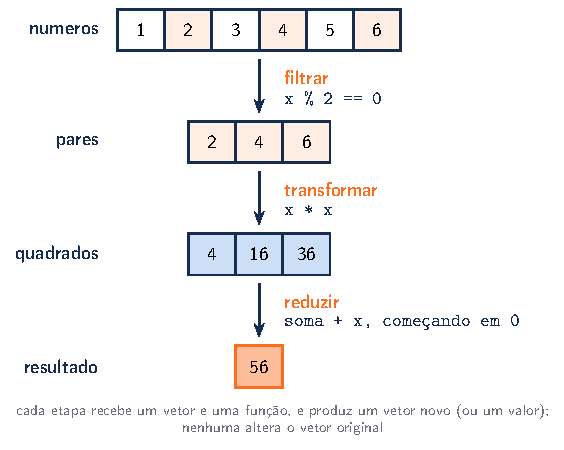
\includegraphics[width=0.75\linewidth,keepaspectratio]{imagens/capitulo-10_pipeline.pdf}
\end{center}

\begin{codigo}
\begin{Verbatim}[breaklines=true, breaksymbolleft={}, fontsize=\footnotesize]
#include <vector>
#include <numeric>     // accumulate
#include <algorithm>   // copy_if, transform
#include <iterator>    // back_inserter

int main() {
    const vector<int> numeros = {1, 2, 3, 4, 5, 6};

    // imperativo: diz COMO fazer, passo a passo
    int soma = 0;
    for (int x : numeros) {
        if (x % 2 == 0) soma += x * x;
    }
    cout << soma << endl;                          // 56

    // funcional: diz O QUE fazer, em etapas
    vector<int> pares, quadrados;
    copy_if(numeros.begin(), numeros.end(),
            back_inserter(pares),
            [](int x) { return x % 2 == 0; });     // filtrar
    transform(pares.begin(), pares.end(),
              back_inserter(quadrados),
              [](int x) { return x * x; });        // transformar
    cout << accumulate(quadrados.begin(), quadrados.end(), 0)
         << endl;                                  // 56: reduzir
}
\end{Verbatim}
\end{codigo}

As expressões entre colchetes, como \texttt{[](int x) \{ return x * x; \}}, são \textbf{lambdas}: funções sem nome, escritas no lugar onde são usadas. O \texttt{back\_inserter(pares)} faz cada elemento produzido ser acrescentado ao fim de \texttt{pares} com \texttt{push\_back}.

Nesse exemplo pequeno, o laço é mais curto. A vantagem do estilo funcional aparece quando as etapas ficam complexas: cada uma é uma peça pequena, com um nome que diz o que faz, que pode ser testada sozinha e reaproveitada em outros lugares. Em C++ os dois estilos convivem, e saber quando usar cada um é parte do trabalho.

\subsection{10.2 Funções puras e imutabilidade}

Uma função é \textbf{pura} quando cumpre duas condições:

\begin{itemize}
  \item o resultado depende \textbf{só dos parâmetros}: chamada com os mesmos argumentos, devolve sempre o mesmo valor;
  \item ela \textbf{não tem efeitos colaterais}: não altera variáveis globais, não modifica os parâmetros, não escreve na tela nem em arquivos.
\end{itemize}

\begin{codigo}
\begin{Verbatim}[breaklines=true, breaksymbolleft={}, fontsize=\footnotesize]
#include <vector>

int total = 0;                    // estado global

// impura: depende de algo de fora e o altera
int somarAoTotal(int x) {
    total += x;
    return total;
}

// pura: o resultado depende só dos parâmetros
int somar(int a, int b) {
    return a + b;
}

// impura: altera o vetor recebido
void dobrarNoLugar(vector<int> &v) {
    for (int &x : v) x *= 2;
}

// pura: devolve um vetor novo e não mexe no original
vector<int> dobrado(const vector<int> &v) {
    vector<int> resultado;
    for (int x : v) resultado.push_back(x * 2);
    return resultado;
}

int main() {
    int a = somarAoTotal(5);
    int b = somarAoTotal(5);
    cout << a << " " << b << endl;   // 5 10: mesma chamada!
    cout << somar(2, 3) << " " << somar(2, 3) << endl;   // 5 5

    const vector<int> original = {1, 2, 3};
    vector<int> novo = dobrado(original);
    cout << original[0] << " " << novo[0] << endl;       // 1 2

    vector<int> copia = original;
    dobrarNoLugar(copia);
    cout << copia[2] << endl;                            // 6
}
\end{Verbatim}
\end{codigo}

Funções puras são mais fáceis de entender, porque basta olhar para elas mesmas, sem procurar quem mais mexe em cada variável. São mais fáceis de \textbf{testar}, como você verá no Capítulo 11: basta comparar a saída com o valor esperado. Podem ter o resultado \textbf{memorizado}, como na programação dinâmica do Capítulo 9, já que a mesma entrada sempre dá a mesma saída. E podem rodar \textbf{em paralelo} sem risco, porque não disputam nenhuma variável.

Um programa útil, claro, precisa ler dados e mostrar resultados, e isso é efeito colateral. A ideia não é eliminá-los, e sim \textbf{isolá-los}: concentrar a entrada e a saída em poucos pontos, como o \texttt{main}, e deixar os cálculos em funções puras.

\subsubsection{Imutabilidade}

A outra metade da ideia é a \textbf{imutabilidade}: em vez de alterar um valor, crie um novo. Em C++, a ferramenta para isso é o \texttt{const}. Uma variável \texttt{const} não pode ser alterada depois de criada, e um parâmetro \texttt{const vector<int> \&} deixa a função ler o vetor sem copiá-lo e sem poder modificá-lo. O compilador recusa qualquer tentativa de alteração, então o erro aparece na compilação e não durante a execução.

Criar valores novos tem um custo: \texttt{dobrado} aloca um vetor inteiro, enquanto \texttt{dobrarNoLugar} não aloca nada. Em vetores enormes, ou em laços que rodam milhões de vezes, a versão que altera no lugar pode ser necessária. A regra prática é usar \texttt{const} sempre que possível e abrir mão da imutabilidade só quando houver um motivo concreto.

\subsection{10.3 Funções como valores}

Na programação funcional, funções são valores como quaisquer outros: podem ser guardadas em variáveis, passadas como parâmetro e devolvidas por outras funções. Em C++, o jeito mais prático de criar uma função no meio do código é a lambda:

\begin{center}
\texttt{[captura](parâmetros) -> tipo de retorno \{ corpo \}}
\end{center}

\begin{itemize}
  \item A \textbf{captura}, entre colchetes, diz quais variáveis de fora a lambda pode usar (Seção 10.4). Os colchetes vazios significam ``nenhuma''.
  \item Os \textbf{parâmetros} e o \textbf{corpo} são os de uma função comum.
  \item O \textbf{tipo de retorno} costuma ser omitido, porque o compilador o deduz do \texttt{return}. Ele só é necessário quando a dedução não é a desejada.
\end{itemize}

Cada lambda tem um tipo próprio, inventado pelo compilador, que não tem nome. Por isso, ela é guardada em uma variável \texttt{auto}. Quando é preciso dar um tipo explícito, por exemplo para guardar lambdas diferentes na mesma variável, usa-se a \texttt{function}, da biblioteca \texttt{<functional>}: \texttt{function<int(int)>} guarda qualquer coisa que possa ser chamada recebendo um \texttt{int} e devolvendo um \texttt{int}.

\begin{codigo}
\begin{Verbatim}[breaklines=true, breaksymbolleft={}, fontsize=\footnotesize]
#include <vector>
#include <functional>   // function

// recebe uma função como parâmetro e a aplica a cada elemento
vector<int> aplicar(const vector<int> &v,
                    const function<int(int)> &f) {
    vector<int> resultado;
    for (int x : v) resultado.push_back(f(x));
    return resultado;
}

int triplo(int x) {                // função comum
    return 3 * x;
}

int main() {
    auto quadrado = [](int x) { return x * x; };
    auto media = [](int a, int b) -> double {  // retorno dado
        return (a + b) / 2.0;
    };
    cout << quadrado(7) << " " << media(6, 9) << endl;  // 49 7.5

    function<int(int)> operacao = quadrado;
    cout << operacao(4) << endl;                // 16
    operacao = [](int x) { return -x; };        // outra lambda
    cout << operacao(4) << endl;                // -4

    vector<int> v = {1, 2, 3};
    for (int x : aplicar(v, quadrado)) cout << x << " ";
    for (int x : aplicar(v, triplo)) cout << x << " ";
    cout << endl;                               // 1 4 9 3 6 9
}
\end{Verbatim}
\end{codigo}

A função \texttt{aplicar} aceita tanto uma lambda quanto uma função comum, como \texttt{triplo}: para a \texttt{function}, basta que a coisa possa ser chamada do jeito certo. Uma função que recebe ou devolve outras funções é chamada de \textbf{função de ordem superior}.

\subsection{10.4 Capturas e \textit{closures}}

Uma lambda com colchetes vazios só enxerga os próprios parâmetros. Para usar uma variável de fora, ela precisa \textbf{capturá-la}, e há dois jeitos:

\begin{itemize}
  \item \textbf{Por valor}, \texttt{[taxa]}: a lambda guarda uma \textbf{cópia} da variável, feita no momento em que é criada. Mudanças posteriores na original não a afetam.
  \item \textbf{Por referência}, \texttt{[\&taxa]}: a lambda guarda uma \textbf{referência} para a variável original e sempre enxerga o valor atual dela.
\end{itemize}

\begin{center}
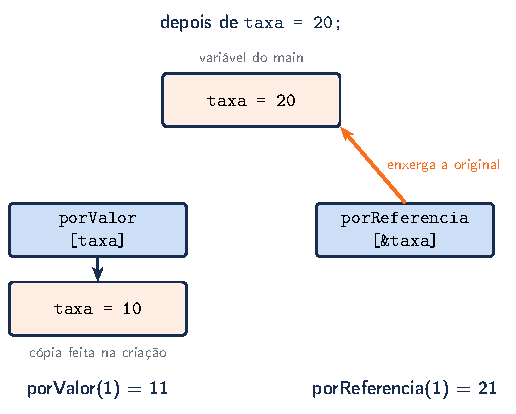
\includegraphics[width=0.7\linewidth,keepaspectratio]{imagens/capitulo-10_captura.pdf}
\end{center}

Uma lambda junto com as variáveis que capturou é chamada de \textbf{\textit{closure}} (fechamento). Ela permite criar funções ``configuradas'': uma função que devolve uma lambda, capturando os próprios parâmetros, funciona como uma fábrica de funções.

\begin{codigo}
\begin{Verbatim}[breaklines=true, breaksymbolleft={}, fontsize=\footnotesize]
#include <functional>

// fábrica: devolve uma função que soma n ao argumento
function<int(int)> somador(int n) {
    return [n](int x) { return x + n; };   // copia o n
}

// cada contador criado guarda a própria contagem
function<int()> criarContador() {
    int contagem = 0;
    return [contagem]() mutable { return ++contagem; };
}

int main() {
    int taxa = 10;
    auto porValor = [taxa](int x) { return x + taxa; };
    auto porReferencia = [&taxa](int x) { return x + taxa; };
    taxa = 20;
    cout << porValor(1) << " " << porReferencia(1) << endl;
    // 11 21

    auto mais5 = somador(5);
    auto mais100 = somador(100);
    cout << mais5(1) << " " << mais100(1) << endl;   // 6 101

    auto c1 = criarContador();
    auto c2 = criarContador();
    c1();
    c1();
    cout << c1() << " " << c2() << endl;             // 3 1
}
\end{Verbatim}
\end{codigo}

Por padrão, as cópias capturadas por valor são \texttt{const} dentro da lambda. Para alterá-las, como faz o contador, a lambda precisa ser marcada com \texttt{mutable}. Cada chamada a \texttt{criarContador} cria uma lambda nova, com a própria cópia de \texttt{contagem}: por isso \texttt{c1} e \texttt{c2} contam separadamente.

Existem também as capturas automáticas: \texttt{[=]} captura por valor tudo o que a lambda usar, e \texttt{[\&]}, tudo por referência. Elas são práticas, mas escondem o que está sendo capturado; prefira listar as variáveis.

\begin{destaque}{Cuidado com a referência que morre}
Uma variável local deixa de existir quando a função termina. Se uma lambda capturar essa variável por referência e for devolvida, ela vai apontar para uma memória que já foi liberada, o mesmo problema de um ponteiro usado depois do \texttt{delete}, visto no Capítulo 1. O comentário \texttt{ERRADO!} marca a linha: o \texttt{n} deixa de existir assim que \texttt{somadorErrado} termina. O programa compila, mas o resultado é imprevisível:

\begin{codigo}
\begin{Verbatim}[breaklines=true, breaksymbolleft={}, fontsize=\footnotesize]
// trecho
function<int(int)> somadorErrado(int n) {
    return [&n](int x) { return x + n; };   // ERRADO!
}
\end{Verbatim}
\end{codigo}

A regra: lambdas que vão sobreviver à função onde foram criadas devem capturar \textbf{por valor}.
\end{destaque}

\subsection{10.5 Mapear, filtrar e reduzir}

Três funções de ordem superior resolvem uma parte enorme dos problemas com coleções:

\begin{itemize}
  \item \textbf{mapear} (\textit{map}): aplica uma função a cada elemento e devolve a coleção dos resultados;
  \item \textbf{filtrar} (\textit{filter}): devolve só os elementos para os quais uma função responde \texttt{true};
  \item \textbf{reduzir} (\textit{reduce} ou \textit{fold}): combina todos os elementos em um único valor, usando uma função que junta o valor acumulado com o próximo elemento.
\end{itemize}

Para ver que não há mágica nelas, o programa abaixo implementa as três com \textit{templates} (Capítulo 1) e as usa para analisar as notas de uma turma. O tipo do vetor devolvido por \texttt{mapear} é o tipo do que a função \texttt{f} devolve, obtido com \texttt{decltype}, que dá o tipo de uma expressão sem executá-la.

\begin{codigo}
\begin{Verbatim}[breaklines=true, breaksymbolleft={}, fontsize=\footnotesize]
#include <vector>

template <typename T, typename F>
auto mapear(const vector<T> &v, F f) {
    vector<decltype(f(v[0]))> resultado;
    for (const T &x : v) resultado.push_back(f(x));
    return resultado;
}

template <typename T, typename F>
vector<T> filtrar(const vector<T> &v, F manter) {
    vector<T> resultado;
    for (const T &x : v) {
        if (manter(x)) resultado.push_back(x);
    }
    return resultado;
}

template <typename T, typename A, typename F>
A reduzir(const vector<T> &v, A inicial, F juntar) {
    A acumulado = inicial;
    for (const T &x : v) acumulado = juntar(acumulado, x);
    return acumulado;
}

struct Aluno {
    string nome;
    double nota;
};

int main() {
    const vector<Aluno> turma = {{"Ana", 8.5}, {"Bruno", 5.0},
                                 {"Carla", 9.0}, {"Davi", 4.5},
                                 {"Eva", 7.0}};
    auto aprovados = filtrar(turma, [](const Aluno &a) {
        return a.nota >= 6;
    });
    auto nomes = mapear(aprovados, [](const Aluno &a) {
        return a.nome;
    });
    double soma = reduzir(turma, 0.0,
                          [](double s, const Aluno &a) {
                              return s + a.nota;
                          });
    for (const string &nome : nomes) cout << nome << " ";
    cout << endl;                                 // Ana Carla Eva
    cout << soma / turma.size() << endl;          // 6.8
}
\end{Verbatim}
\end{codigo}

Repare no \texttt{0.0} passado a \texttt{reduzir}: o tipo do valor inicial é o tipo do acumulado. Com \texttt{0}, um \texttt{int}, as notas seriam somadas como inteiros e as casas decimais se perderiam.

\subsubsection{As versões da biblioteca padrão}

A biblioteca \texttt{<algorithm>} (e a \texttt{<numeric>}, para a redução) traz versões prontas dessas funções e de várias outras. Elas trabalham com iteradores, como as buscas do Capítulo 7:

\begin{center}
\begin{tabular}{@{}p{0.3\linewidth}p{0.6\linewidth}@{}}
\toprule
\rowcolor{headergray}
\tblheader{Função} & \tblheader{O que faz} \\
\midrule
\texttt{transform} & mapear: aplica a função e grava os resultados no destino \\
\rowcolor{rowgray} \texttt{copy\_if} & filtrar: copia para o destino os que passam no teste \\
\texttt{accumulate} & reduzir: combina tudo a partir de um valor inicial (soma, se nenhuma função for dada) \\
\rowcolor{rowgray} \texttt{count\_if} & conta quantos passam no teste \\
\texttt{all\_of}, \texttt{any\_of}, \texttt{none\_of} & todos, algum ou nenhum passa no teste? \\
\rowcolor{rowgray} \texttt{find\_if} & primeiro que passa no teste \\
\texttt{max\_element}, \texttt{min\_element} & maior ou menor, segundo um critério \\
\rowcolor{rowgray} \texttt{for\_each} & executa a função para cada elemento \\
\bottomrule
\end{tabular}
\end{center}

\begin{codigo}
\begin{Verbatim}[breaklines=true, breaksymbolleft={}, fontsize=\footnotesize]
#include <vector>
#include <algorithm>
#include <numeric>     // accumulate

struct Aluno {
    string nome;
    double nota;
};

int main() {
    const vector<Aluno> turma = {{"Ana", 8.5}, {"Bruno", 5.0},
                                 {"Carla", 9.0}, {"Davi", 4.5},
                                 {"Eva", 7.0}};
    auto reprovado = [](const Aluno &a) { return a.nota < 6; };

    cout << count_if(turma.begin(), turma.end(), reprovado)
         << " reprovados" << endl;                 // 2 reprovados

    bool todosAcimaDe4 = all_of(turma.begin(), turma.end(),
        [](const Aluno &a) { return a.nota > 4; });
    bool algumDez = any_of(turma.begin(), turma.end(),
        [](const Aluno &a) { return a.nota == 10; });
    cout << boolalpha << todosAcimaDe4 << " " << algumDez
         << endl;                                  // true false

    auto melhor = max_element(turma.begin(), turma.end(),
        [](const Aluno &a, const Aluno &b) {
            return a.nota < b.nota;          // "a vem antes"
        });
    cout << melhor->nome << endl;                  // Carla

    double soma = accumulate(turma.begin(), turma.end(), 0.0,
        [](double s, const Aluno &a) { return s + a.nota; });
    cout << soma << endl;                          // 34
}
\end{Verbatim}
\end{codigo}

A lambda \texttt{reprovado} foi guardada em uma variável e usada pelo nome, o que deixa a linha do \texttt{count\_if} quase uma frase em português. Dar nomes às condições é uma das formas mais simples de tornar o código legível.

\subsection{10.6 Composição de funções}

\textbf{Compor} duas funções é criar uma terceira que aplica uma e depois a outra: a composta de \texttt{f} com \texttt{g} é a função que leva \texttt{x} a \texttt{f(g(x))}. Como funções são valores, a composição também pode ser escrita como uma função de ordem superior, que recebe duas funções e devolve uma nova.

\begin{codigo}
\begin{Verbatim}[breaklines=true, breaksymbolleft={}, fontsize=\footnotesize]
#include <string>
#include <algorithm>   // transform, remove
#include <cctype>      // tolower

// devolve a função x -> f(g(x)): primeiro g, depois f
template <typename F, typename G>
auto compor(F f, G g) {
    return [f, g](auto x) { return f(g(x)); };
}

int main() {
    auto dobro = [](int x) { return 2 * x; };
    auto maisUm = [](int x) { return x + 1; };
    auto h1 = compor(maisUm, dobro);    // 2x + 1
    auto h2 = compor(dobro, maisUm);    // 2(x + 1)
    cout << h1(5) << " " << h2(5) << endl;   // 11 12

    auto semEspacos = [](string s) {
        s.erase(remove(s.begin(), s.end(), ' '), s.end());
        return s;
    };
    auto minusculas = [](string s) {
        transform(s.begin(), s.end(), s.begin(),
                  [](unsigned char c) { return tolower(c); });
        return s;
    };
    auto normalizarEmail = compor(minusculas, semEspacos);
    cout << normalizarEmail(" Ana.Silva@Email.COM ") << endl;
    // ana.silva@email.com
}
\end{Verbatim}
\end{codigo}

A ordem importa: \texttt{h1} e \texttt{h2} combinam as mesmas duas funções e dão resultados diferentes. O parâmetro \texttt{auto x} faz da lambda devolvida uma \textbf{lambda genérica}, que aceita qualquer tipo, como um \textit{template}; por isso a mesma \texttt{compor} serve para números e para textos.

As lambdas \texttt{semEspacos} e \texttt{minusculas} recebem a \texttt{string} por valor e devolvem a cópia alterada, sem mexer no texto original: são funções puras, mesmo alterando uma variável internamente. A linha com \texttt{erase} e \texttt{remove} é a forma padrão de apagar elementos de um vetor ou texto em C++: a \texttt{remove} empurra para o fim os que devem sair, e a \texttt{erase} corta esse fim.

\begin{destaque}{Ranges no C++20}
As versões mais novas do C++ (a partir do C++20) trazem as \textit{ranges}, que permitem encadear as etapas com o operador \texttt{|}, de forma parecida com uma linha de comandos: \texttt{numeros | views::filter(par) | views::transform(quadrado)}. As etapas são \textbf{preguiçosas}: nada é calculado nem copiado até que os elementos sejam percorridos. Esta apostila usa o C++17, mas vale saber que o estilo funcional em C++ continua evoluindo nessa direção.
\end{destaque}

\subsection{10.7 Quando usar o estilo funcional}

\begin{center}
\begin{tabular}{@{}p{0.45\linewidth}p{0.45\linewidth}@{}}
\toprule
\rowcolor{headergray}
\tblheader{Combina bem} & \tblheader{Combina menos} \\
\midrule
transformar, filtrar e resumir coleções & laços com muitas condições de parada e casos especiais \\
\rowcolor{rowgray} regras de negócio e cálculos que podem ser funções puras & código cujo trabalho é o efeito colateral: ler, gravar, desenhar \\
critérios de ordenação, busca e contagem & trechos em que copiar dados a cada etapa custaria caro \\
\rowcolor{rowgray} código que precisa ser testado ou rodar em paralelo & equipes que ainda não conhecem o estilo \\
\bottomrule
\end{tabular}
\end{center}

O objetivo não é eliminar laços nem variáveis, mas ter mais uma ferramenta. Na prática, um bom programa C++ costuma misturar os dois estilos: estruturas de dados e entrada e saída escritas de forma imperativa, e cálculos e transformações escritos com funções puras e algoritmos da biblioteca.

\begin{destaque}{Comparando com Python}
Em Python, funções também são valores, e a palavra \texttt{lambda} cria funções anônimas de uma única expressão. As funções \texttt{map} e \texttt{filter} são nativas, e a \texttt{reduce} está no módulo \texttt{functools}. Mas o jeito mais comum de mapear e filtrar em Python são as \textbf{compreensões de lista}, que fazem as duas coisas em uma linha.

\begin{codigo}
\begin{Verbatim}[breaklines=true, breaksymbolleft={}, fontsize=\footnotesize]
from functools import reduce

numeros = [1, 2, 3, 4, 5, 6]
pares = filter(lambda x: x % 2 == 0, numeros)
quadrados = map(lambda x: x * x, pares)
print(reduce(lambda soma, x: soma + x, quadrados, 0))   # 56

print(sum(x * x for x in numeros if x % 2 == 0))   # 56
print([x * x for x in numeros if x % 2 == 0])      # [4, 16, 36]

def somador(n):
    return lambda x: x + n        # closure: guarda o n

mais5 = somador(5)
print(mais5(1))                   # 6

def criar_contador():
    contagem = 0
    def contar():
        nonlocal contagem         # altera a variável de fora
        contagem += 1
        return contagem
    return contar

c1 = criar_contador()
c1()
c1()
print(c1())                       # 3
\end{Verbatim}
\end{codigo}

Em Python, \texttt{map} e \texttt{filter} são preguiçosas, como as \textit{ranges} do C++20: elas só calculam quando alguém percorre o resultado. A palavra \texttt{nonlocal} tem o papel do \texttt{mutable} do C++: sem ela, \texttt{contagem += 1} criaria uma variável local nova em vez de alterar a capturada. E, diferente do C++, as closures do Python sempre enxergam a variável original, como uma captura por referência.
\end{destaque}

\subsection{Erros Comuns}

\begin{itemize}
  \item \textbf{Devolver uma lambda que captura uma variável local por referência.} A variável deixa de existir quando a função termina, e a lambda passa a ler lixo. Capture por valor.
  \item \textbf{Esperar que a captura por valor acompanhe a variável.} A cópia é feita quando a lambda é criada; alterações posteriores na variável original não aparecem nela.
  \item \textbf{Esquecer o \texttt{mutable}.} Sem ele, alterar uma variável capturada por valor é erro de compilação.
  \item \textbf{Esquecer de capturar.} Uma lambda com \texttt{[]} não enxerga as variáveis locais de fora; usá-las dá erro de compilação.
  \item \textbf{Usar \texttt{transform} ou \texttt{copy\_if} com um destino vazio.} Sem o \texttt{back\_inserter}, elas escrevem por cima de posições que não existem. Use \texttt{back\_inserter} ou reserve o tamanho antes.
  \item \textbf{Passar \texttt{0} como valor inicial do \texttt{accumulate} para somar \texttt{double}.} O resultado é calculado como \texttt{int} e perde as casas decimais. Use \texttt{0.0}.
  \item \textbf{Chamar de pura uma função que mostra coisas na tela ou altera globais.} Esses efeitos colaterais quebram as vantagens da função pura, como poder testá-la e memorizá-la.
  \item \textbf{Encadear etapas demais em uma única expressão.} Uma linha com cinco lambdas aninhadas é mais difícil de ler que um laço. Dê nomes às etapas e às condições.
\end{itemize}
